\begin{frame}{Trabajar con Remotos}
  \begin{itemize}
    \item \alert{Ver tus remotos}
      \mint{console}| $ git remote -v|
    \item \alert{Añadir un remoto}
      \mint{console}| $ git remote add <nombre-remoto> <url>|
    \item \alert{Inspeccionar un remoto}
      \mint{console}| $ git remote show <nombre-remoto>|
    \item \alert{Eliminar un remoto}
      \mint{console}| $ git remote rm <nombre-remoto>|
    \item \alert{Renombrar un remoto}
      \mint{console}| $ git remote rename <nombre> <nombre-nuevo>|
  \end{itemize}
\end{frame}

\begin{frame}{Trabajar con Remotos}
  \begin{itemize}
    \item \alert{Traer remotos}
      \mint{console}| $ git fetch <nombre-remoto>|
      Creará una nueva rama con el trabajo del remoto
    \item \alert{Traer y Combinar remotos}
      \mint{console}| $ git pull <nombre-remoto> <nombre-rama>|
      \texttt{push = fetch + merge}
    \item \alert{Enviar a tus remotos}
      \mint{console}| $ git push <nombre-remoto> <nombre-rama>|
  \end{itemize}
  Si nuestra rama rastrea la rama remota, se puede no especificar nombres
  \begin{tikzpicture}[remember picture,overlay]
    \node[anchor=north east,inner ysep=50pt, inner xsep=20pt] at (current page.north east) {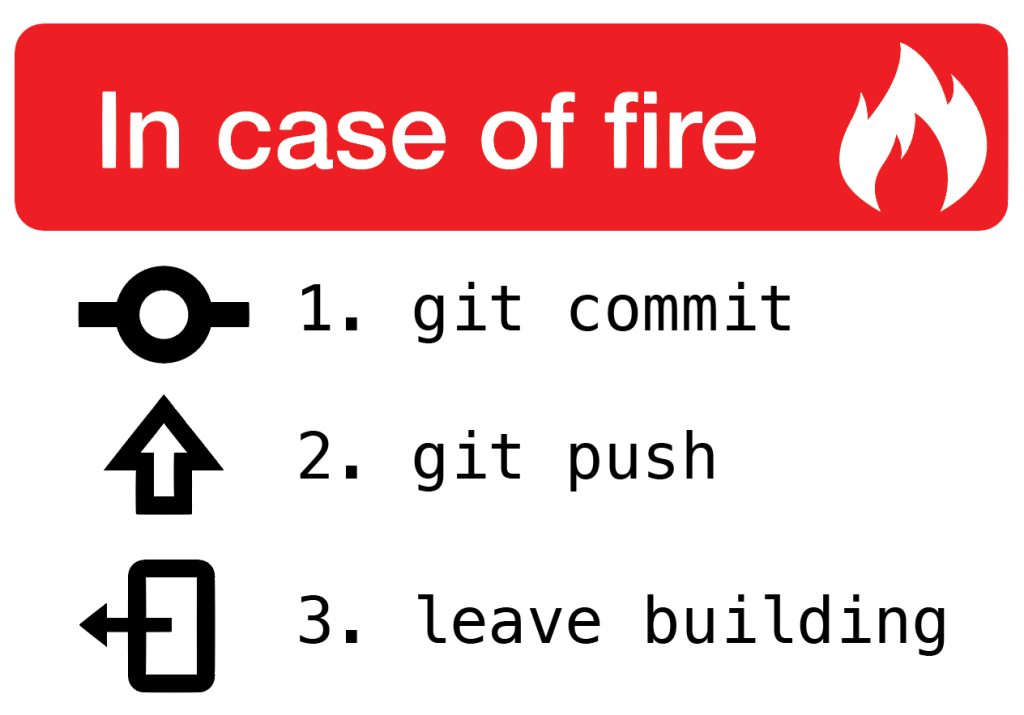
\includegraphics[scale=0.5]{images/incaseoffire.png}};
  \end{tikzpicture}
\end{frame}
